% Options for packages loaded elsewhere
\PassOptionsToPackage{unicode}{hyperref}
\PassOptionsToPackage{hyphens}{url}
\PassOptionsToPackage{dvipsnames,svgnames,x11names}{xcolor}
%
\documentclass[
  letterpaper,
  DIV=11,
  numbers=noendperiod]{scrartcl}

\usepackage{amsmath,amssymb}
\usepackage{iftex}
\ifPDFTeX
  \usepackage[T1]{fontenc}
  \usepackage[utf8]{inputenc}
  \usepackage{textcomp} % provide euro and other symbols
\else % if luatex or xetex
  \usepackage{unicode-math}
  \defaultfontfeatures{Scale=MatchLowercase}
  \defaultfontfeatures[\rmfamily]{Ligatures=TeX,Scale=1}
\fi
\usepackage{lmodern}
\ifPDFTeX\else  
    % xetex/luatex font selection
\fi
% Use upquote if available, for straight quotes in verbatim environments
\IfFileExists{upquote.sty}{\usepackage{upquote}}{}
\IfFileExists{microtype.sty}{% use microtype if available
  \usepackage[]{microtype}
  \UseMicrotypeSet[protrusion]{basicmath} % disable protrusion for tt fonts
}{}
\makeatletter
\@ifundefined{KOMAClassName}{% if non-KOMA class
  \IfFileExists{parskip.sty}{%
    \usepackage{parskip}
  }{% else
    \setlength{\parindent}{0pt}
    \setlength{\parskip}{6pt plus 2pt minus 1pt}}
}{% if KOMA class
  \KOMAoptions{parskip=half}}
\makeatother
\usepackage{xcolor}
\setlength{\emergencystretch}{3em} % prevent overfull lines
\setcounter{secnumdepth}{-\maxdimen} % remove section numbering
% Make \paragraph and \subparagraph free-standing
\makeatletter
\ifx\paragraph\undefined\else
  \let\oldparagraph\paragraph
  \renewcommand{\paragraph}{
    \@ifstar
      \xxxParagraphStar
      \xxxParagraphNoStar
  }
  \newcommand{\xxxParagraphStar}[1]{\oldparagraph*{#1}\mbox{}}
  \newcommand{\xxxParagraphNoStar}[1]{\oldparagraph{#1}\mbox{}}
\fi
\ifx\subparagraph\undefined\else
  \let\oldsubparagraph\subparagraph
  \renewcommand{\subparagraph}{
    \@ifstar
      \xxxSubParagraphStar
      \xxxSubParagraphNoStar
  }
  \newcommand{\xxxSubParagraphStar}[1]{\oldsubparagraph*{#1}\mbox{}}
  \newcommand{\xxxSubParagraphNoStar}[1]{\oldsubparagraph{#1}\mbox{}}
\fi
\makeatother


\providecommand{\tightlist}{%
  \setlength{\itemsep}{0pt}\setlength{\parskip}{0pt}}\usepackage{longtable,booktabs,array}
\usepackage{calc} % for calculating minipage widths
% Correct order of tables after \paragraph or \subparagraph
\usepackage{etoolbox}
\makeatletter
\patchcmd\longtable{\par}{\if@noskipsec\mbox{}\fi\par}{}{}
\makeatother
% Allow footnotes in longtable head/foot
\IfFileExists{footnotehyper.sty}{\usepackage{footnotehyper}}{\usepackage{footnote}}
\makesavenoteenv{longtable}
\usepackage{graphicx}
\makeatletter
\newsavebox\pandoc@box
\newcommand*\pandocbounded[1]{% scales image to fit in text height/width
  \sbox\pandoc@box{#1}%
  \Gscale@div\@tempa{\textheight}{\dimexpr\ht\pandoc@box+\dp\pandoc@box\relax}%
  \Gscale@div\@tempb{\linewidth}{\wd\pandoc@box}%
  \ifdim\@tempb\p@<\@tempa\p@\let\@tempa\@tempb\fi% select the smaller of both
  \ifdim\@tempa\p@<\p@\scalebox{\@tempa}{\usebox\pandoc@box}%
  \else\usebox{\pandoc@box}%
  \fi%
}
% Set default figure placement to htbp
\def\fps@figure{htbp}
\makeatother

\usepackage{booktabs}
\usepackage{longtable}
\usepackage{array}
\usepackage{multirow}
\usepackage{wrapfig}
\usepackage{float}
\usepackage{colortbl}
\usepackage{pdflscape}
\usepackage{tabu}
\usepackage{threeparttable}
\usepackage{threeparttablex}
\usepackage[normalem]{ulem}
\usepackage{makecell}
\usepackage{xcolor}
\KOMAoption{captions}{tableheading}
\makeatletter
\@ifpackageloaded{caption}{}{\usepackage{caption}}
\AtBeginDocument{%
\ifdefined\contentsname
  \renewcommand*\contentsname{Table of contents}
\else
  \newcommand\contentsname{Table of contents}
\fi
\ifdefined\listfigurename
  \renewcommand*\listfigurename{List of Figures}
\else
  \newcommand\listfigurename{List of Figures}
\fi
\ifdefined\listtablename
  \renewcommand*\listtablename{List of Tables}
\else
  \newcommand\listtablename{List of Tables}
\fi
\ifdefined\figurename
  \renewcommand*\figurename{Figure}
\else
  \newcommand\figurename{Figure}
\fi
\ifdefined\tablename
  \renewcommand*\tablename{Table}
\else
  \newcommand\tablename{Table}
\fi
}
\@ifpackageloaded{float}{}{\usepackage{float}}
\floatstyle{ruled}
\@ifundefined{c@chapter}{\newfloat{codelisting}{h}{lop}}{\newfloat{codelisting}{h}{lop}[chapter]}
\floatname{codelisting}{Listing}
\newcommand*\listoflistings{\listof{codelisting}{List of Listings}}
\makeatother
\makeatletter
\makeatother
\makeatletter
\@ifpackageloaded{caption}{}{\usepackage{caption}}
\@ifpackageloaded{subcaption}{}{\usepackage{subcaption}}
\makeatother

\usepackage{bookmark}

\IfFileExists{xurl.sty}{\usepackage{xurl}}{} % add URL line breaks if available
\urlstyle{same} % disable monospaced font for URLs
\hypersetup{
  pdftitle={Data analysis project 12},
  colorlinks=true,
  linkcolor={blue},
  filecolor={Maroon},
  citecolor={Blue},
  urlcolor={Blue},
  pdfcreator={LaTeX via pandoc}}


\title{Data analysis project 12}
\author{}
\date{}

\begin{document}
\maketitle


\section{Introduction}\label{sec-intro}

Over the years, there has been an increase in the health awareness of
the Scottish population, with a fear that the country as a whole is
becoming overweight. The body mass index (BMI) is a quick way to measure
weight relative to height, and screen for people that are underweight,
overweight, or obese.

This report aims to explore changes in BMI trends in Scotland using data
from the 2013--2016 Scottish Health Survey. Specifically, we seek to
answer the following key questions:

\begin{enumerate}
\def\labelenumi{\arabic{enumi}.}
\tightlist
\item
  Has the BMI in Scotland changed over the given years of the Scottish
  Health Survey?
\item
  Are there any difference inthe BMI distributions by age, gender,
  socioeconomic status or lifestyle factors?
\end{enumerate}

By analyzing this data, we aim to identify patterns that could inform
public health strategies and address potential risk factors contributing
to obesity.

\section{Exploratory data analysis}\label{sec-expdata}

\subsection{Data Overview}\label{data-overview}

\begin{verbatim}
  Age    Sex               Education Year   BMIgroup
1  48 Female       No qualifications 2016      Obese
2  51   Male        Degree or higher 2016 Overweight
3  48 Female        Degree or higher 2016     Normal
4  16 Female       No qualifications 2016     Normal
5  61   Male Standard grade or equiv 2016     Normal
6  40 Female        Degree or higher 2016     Normal
\end{verbatim}

\begin{verbatim}
Rows: 14,017
Columns: 5
$ Age       <int> 48, 51, 48, 16, 61, 40, 43, 40, 39, 45, 18, 29, 36, 37, 78, ~
$ Sex       <chr> "Female", "Male", "Female", "Female", "Male", "Female", "Mal~
$ Education <chr> "No qualifications", "Degree or higher", "Degree or higher",~
$ Year      <int> 2016, 2016, 2016, 2016, 2016, 2016, 2016, 2016, 2016, 2016, ~
$ BMIgroup  <chr> "Obese", "Overweight", "Normal", "Normal", "Normal", "Normal~
\end{verbatim}

\begin{verbatim}
      Age       Sex Education      Year  BMIgroup 
        0         0         0         0         0 
\end{verbatim}

The dataset consists of 14,017 observations with the following columns:

\textbf{Age}: Age of individuals

\textbf{Sex}: Gender of individuals (Male/Female)

\textbf{Education}: Highest educational qualification

\textbf{Year}: Year of the survey (2013-2016)

\textbf{BMIgroup}: Weight classification group (e.g., Obese, Overweight,
Normal)

\subsection{Summary Statistics}\label{summary-statistics}

Computing descriptive statistics helps understand the distribution of
the data.

\begin{longtable}[t]{rrrrrrrr}
\caption{Summary Statistics of the Dataset}\\
\toprule
Sample\_Size & Mean\_Age & Median\_Age & Min\_Age & Q1\_Age & Q3\_Age & Max\_Age & Std\_Age\\
\midrule
14017 & 50.84262 & 51 & 16 & 37 & 65 & 99 & 17.60925\\
\bottomrule
\end{longtable}

Key observations from the summary statistics:

\begin{itemize}
\item
  No missing values are detected.
\item
  Age distribution is fairly wide, with a range from young adults to
  elderly individuals.
\item
  BMI categories contain multiple classifications, which will later be
  converted into a binary variable for analysis.
\end{itemize}

\subsection{Identifying Distribution and Checking
Normality}\label{identifying-distribution-and-checking-normality}

We use a histogram to visualize the distribution of age and assess
normality.

\pandocbounded{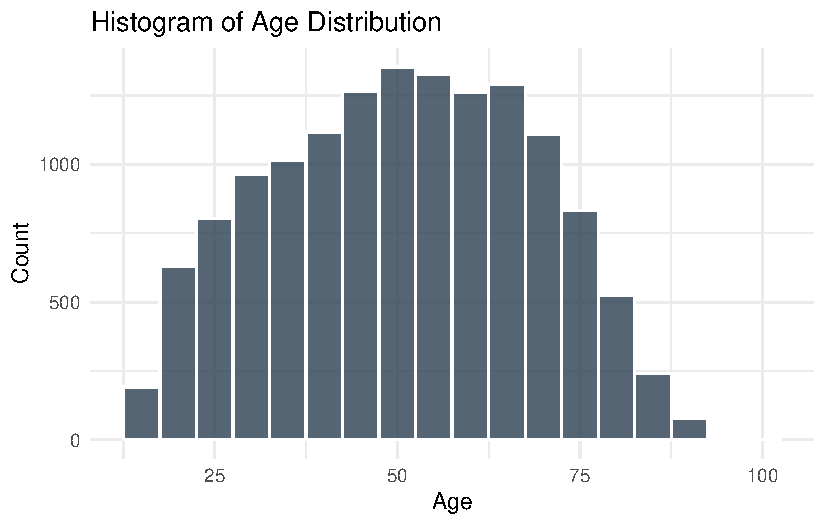
\includegraphics[keepaspectratio]{Data-analysis-12--1---1-_files/figure-pdf/unnamed-chunk-4-1.pdf}}

The histogram reveals that the age distribution in the dataset is
approximately~bell-shaped~but slightly~right-skewed. The majority of
individuals fall within the~40-60 age range, while younger individuals
(\textless20 years) and older individuals (\textgreater80 years) are
less represented. The right skew suggests that there are more older
individuals in the dataset than younger ones.

\subsection{Identifying outliers:}\label{identifying-outliers}

To detect outliers, we use a~boxplot~to visualize the spread of ages
within each~

\pandocbounded{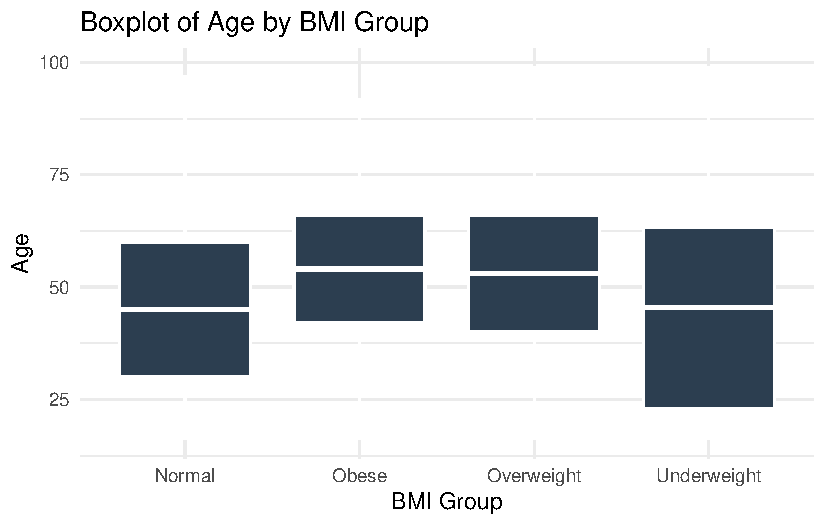
\includegraphics[keepaspectratio]{Data-analysis-12--1---1-_files/figure-pdf/unnamed-chunk-5-1.pdf}}

The boxplot provides a visual summary of the distribution of~age across
different BMI categories (Normal, Obese, Overweight, and Underweight).
Key observations include:

\begin{itemize}
\item
  The~median age varies slightly across BMI groups, with individuals
  classified as overweight and obese tending to be older than those in
  the normal or underweight categories.
\item
  The~interquartile range (IQR)~(middle 50\% of the data) shows that
  most individuals are between~40 and 70 years old, regardless of BMI
  classification.
\item
  There are potential outliers, particularly among~younger and older
  individuals, indicating that some individuals outside the usual age
  range may require further investigation.
\end{itemize}

\subsection{Creating a Binary Obesity
Classification}\label{creating-a-binary-obesity-classification}

Since we want to analyze obesity prevalence, we create a new binary
response variable where:

\begin{itemize}
\item
  Obese = 1
\item
  Not Obese (Normal \& Overweight) = 0
\end{itemize}

\begin{verbatim}

   0    1 
9754 4263 
\end{verbatim}

\subsection{BMI Trends Over Time}\label{bmi-trends-over-time}

Analyzing how obesity has changed over time using proportions.

\pandocbounded{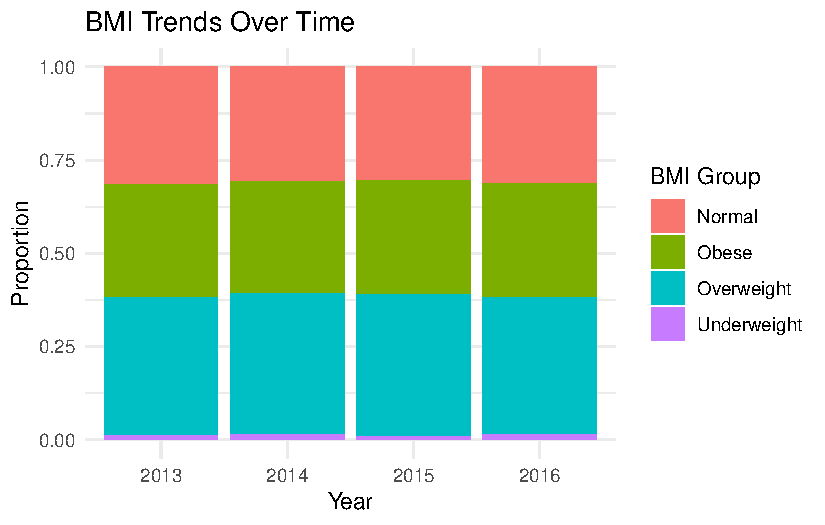
\includegraphics[keepaspectratio]{Data-analysis-12--1---1-_files/figure-pdf/unnamed-chunk-7-1.pdf}}

Key findings:

\begin{itemize}
\item
  The proportion of obese individuals appears relatively stable over the
  years.
\item
  A significant proportion of individuals are classified as overweight.
\end{itemize}

\subsection{Obesity Distribution by
Demographics}\label{obesity-distribution-by-demographics}

\subsubsection{By Age Group}\label{by-age-group}

\pandocbounded{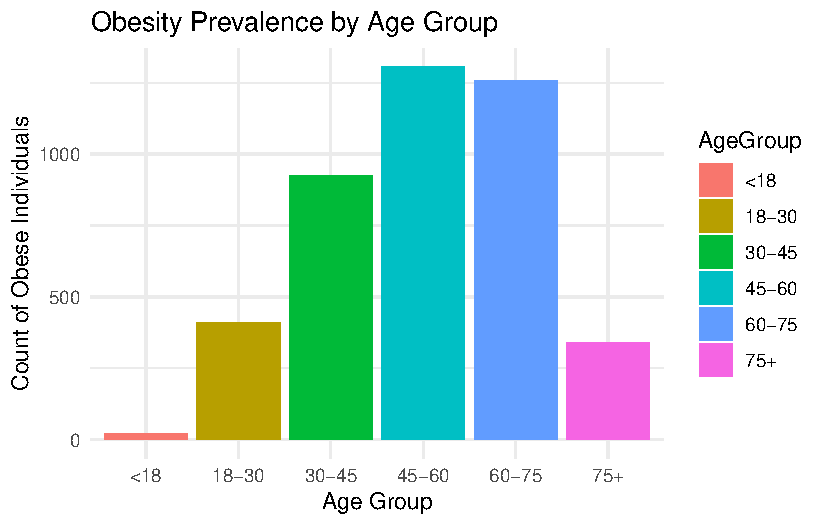
\includegraphics[keepaspectratio]{Data-analysis-12--1---1-_files/figure-pdf/unnamed-chunk-8-1.pdf}}

\begin{itemize}
\tightlist
\item
  Middle-aged individuals (45-60) have the highest obesity rates.
\end{itemize}

\subsubsection{By Gender}\label{by-gender}

\pandocbounded{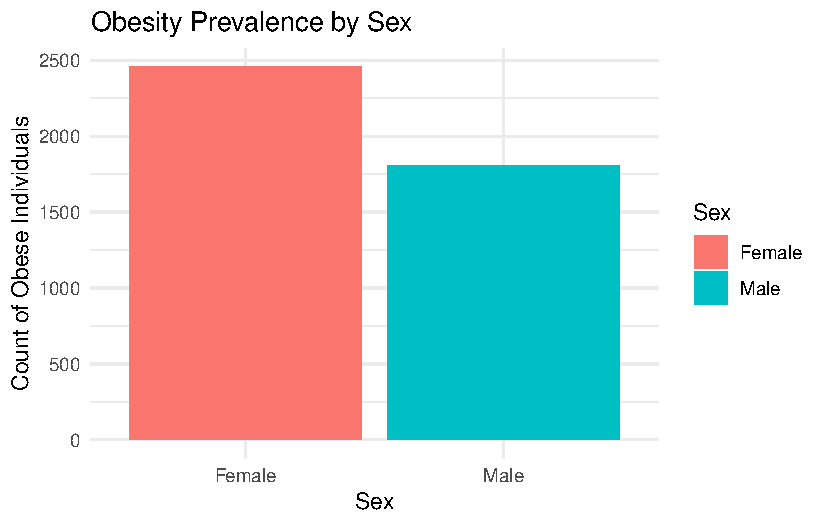
\includegraphics[keepaspectratio]{Data-analysis-12--1---1-_files/figure-pdf/unnamed-chunk-9-1.pdf}}

\begin{itemize}
\tightlist
\item
  Females exhibit higher obesity rates compared to males.
\end{itemize}

\section{Correlation Analysis}\label{correlation-analysis}

Examining the relationship between Age and Obesity.

\begin{verbatim}

    Pearson's product-moment correlation

data:  obesity$Age and obesity$ObeseBinary
t = 11.804, df = 14015, p-value < 2.2e-16
alternative hypothesis: true correlation is not equal to 0
95 percent confidence interval:
 0.08279939 0.11558340
sample estimates:
       cor 
0.09921832 
\end{verbatim}

\pandocbounded{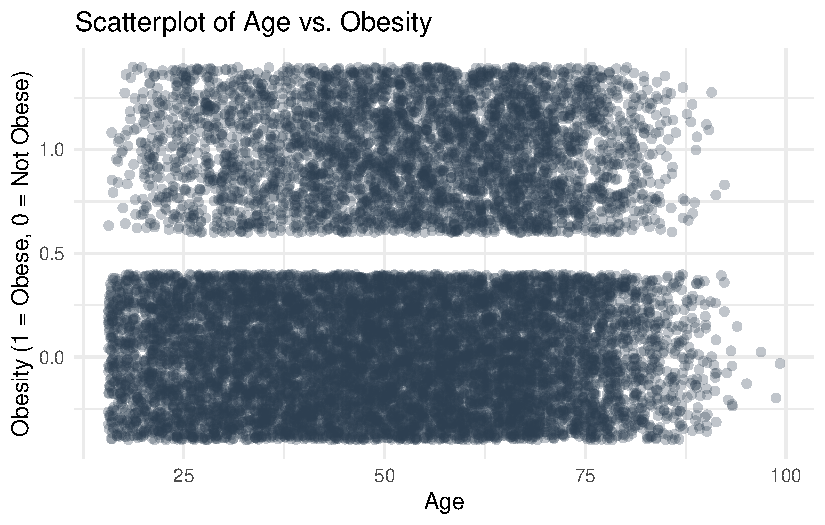
\includegraphics[keepaspectratio]{Data-analysis-12--1---1-_files/figure-pdf/unnamed-chunk-11-1.pdf}}

The scatter plot illustrates the relationship between age and obesity,
where obesity is represented as a binary variable (1= Obese, 0= Not
obese). The distribution of points suggest that obesity is present
across all ages groups without a strong visual trend. The calculated
correlation coefficient of 0.099 indicates a very weak positive
relationship, meaning that as age increases, there is only a slight
tendency for obesity prevalence to rise.

\section{Formal data analysis}\label{sec-formdata}

\begin{longtable}[]{@{}ll@{}}
\toprule\noalign{}
Year & Obese proportions \\
\midrule\noalign{}
\endhead
\bottomrule\noalign{}
\endlastfoot
2013 & 0.30300569 \\
2014 & 0.30181715 \\
2015 & 0.30645161 \\
2016 & 0.30536494 \\
\end{longtable}

\begin{verbatim}
      
       0 1
  2013 3 1
  2014 3 1
  2015 3 1
  2016 3 1
\end{verbatim}

\begin{verbatim}

    Chi-squared Test for Trend in Proportions

data:  trend_table[, 2] out of rowSums(trend_table) ,
 using scores: 1 2 3 4
X-squared = 0, df = 1, p-value = 1
\end{verbatim}

\begin{verbatim}
[1] 2013 2014 2015 2016
\end{verbatim}

\begin{verbatim}
[1] 0 1
\end{verbatim}

\begin{verbatim}

    Pearson's Chi-squared test

data:  trend_table
X-squared = 0, df = 3, p-value = 1
\end{verbatim}

\begin{verbatim}

Call:
glm(formula = obese_binary ~ as.numeric(Year), family = binomial, 
    data = bmi_trends)

Coefficients:
                   Estimate Std. Error z value Pr(>|z|)
(Intercept)      -1.099e+00  1.414e+00  -0.777    0.437
as.numeric(Year) -3.440e-16  5.164e-01   0.000    1.000

(Dispersion parameter for binomial family taken to be 1)

    Null deviance: 17.995  on 15  degrees of freedom
Residual deviance: 17.995  on 14  degrees of freedom
AIC: 21.995

Number of Fisher Scoring iterations: 4
\end{verbatim}

The analysis into whether the prevalence of obesity in Scotland has
changed over the given years of the Scottish Health Survey includes a
Chi-squared test for trend, Pearson's Chi-squared test, and a logistic
regression model.

The Chi-squared test for trend examines whether there is a significant
trend in obesity prevalence over the years. With a test statistic of X²
= 0, df = 1, and a p-value of 1, this suggests no significant trend.

The Pearson's Chi-squared test compares obesity proportions across years
without assuming a trend. With X² = 0, df = 3, and p-value = 1, there is
no significant difference in obesity prevalence across years.

The logistic regression model tests whether the year is a significant
predictor of obesity. The coefficient for year is -9.132e-16 , with a
p-value of 1, indicating no relationship between year and obesity. The
Intercept of -1.099 represents the log-odds of obesity in the baseline
year.

The Akaike Information Criterion (AIC = 21.995) measures model fit, with
lower values indicating better fit. However, since the model finds no
effect of year on obesity, this value is less meaningful in this case.

Overall, all statistical tests confirm that obesity prevalence in
Scotland has remained unchanged over the given years.

\subsubsection{Question 2}\label{question-2}

To answer the second question, we use linear regression to find out if
age, gender, socio-economic status, or lifestyle factors are significant
predictors for obesity.

We start by looking at if age is a significant predictor for a persons
BMI group. We are fitting the following linear model:

\[
logit(\pi) = \beta_0 + \beta_1 x_i + \epsilon_i, ~~~~~ \epsilon_i \sim N(0, \sigma^2), ~~~~~ i = 1, ... , 14017
\]

Here, \(\pi\) is the probability that the individual is obese, \(x_i\)
is the age of the ith individual, and \(\beta_0\), \(\beta_1\) are
regression coefficients. We are using the logit link function.

\begin{longtable}[]{@{}cccc@{}}
\toprule\noalign{}
\endhead
\bottomrule\noalign{}
\endlastfoot
~ & \multicolumn{3}{c@{}}{%
BM Igroup} \\
Predictors & Odds Ratios & CI & p \\
(Intercept) & 4.33 & 3.86~--~4.86 & \textbf{\textless0.001} \\
Age & 0.99 & 0.99~--~0.99 & \textbf{\textless0.001} \\
\end{longtable}

As seen from the p-value, we can infer that age is a significant
predictor for a persons BMI group. As someones age increases by one
year, the odds of the person being obese increase by a factor of 0.99.

We now check the assumptions of our model, to find out if the model is
valid.

\begin{figure}

\centering{

\pandocbounded{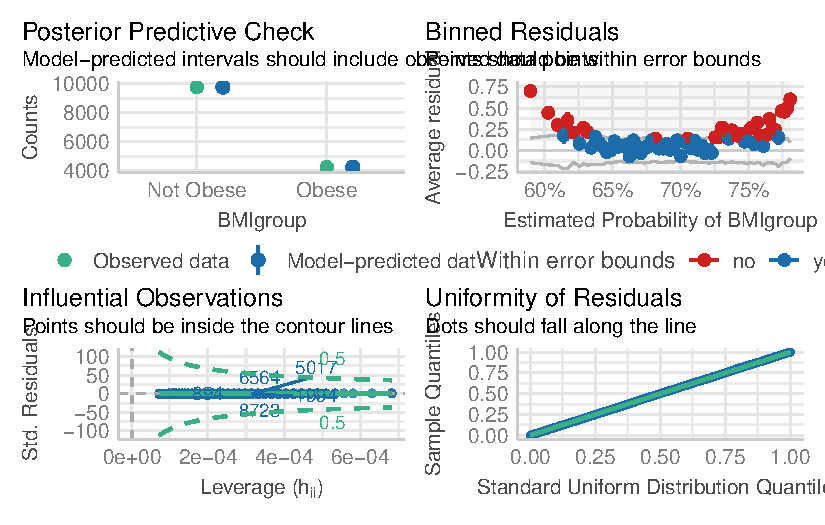
\includegraphics[keepaspectratio]{Data-analysis-12--1---1-_files/figure-pdf/fig-diagnostics1-1.pdf}}

}

\caption{\label{fig-diagnostics1}Diagnostic plots for the age model}

\end{figure}%

There is no issues that can be seen in the posterior predictive check,
influential obesvations graph, and the uniformity of resuduals graph.
There does appear to be a large amount of points falling outiwth the
error bounds in the binned residuals graph. We would expect about 95\%
of points to fall within the error bounds if the model is true. As there
is a large amount of points plotted it is hard to tell if there is 95\%
within the error bounds, as there may be overlap. However, it appears to
be good enough.

We now look at sex to consider if it is significant through fitting the
following model:

\[
logit(\pi) = \beta_0 + \beta_1 x_i + \epsilon_i, ~~~~~ \epsilon_i \sim N(0, \sigma^2), ~~~~~ i = 1, ... , 14017
\]

Where \(x_i\) is an indicator variable taking the value 0 if the
individual is a male and the value 1 if the individual is a female.

\begin{longtable}[]{@{}cccc@{}}
\toprule\noalign{}
\endhead
\bottomrule\noalign{}
\endlastfoot
~ & \multicolumn{3}{c@{}}{%
BM Igroup} \\
Predictors & Odds Ratios & CI & p \\
(Intercept) & 2.44 & 2.31~--~2.57 & \textbf{\textless0.001} \\
Sex {[}Female{]} & 0.89 & 0.83~--~0.96 & \textbf{0.002} \\
R\textsuperscript{2} Tjur & \multicolumn{3}{l@{}}{%
0.001} \\
\end{longtable}

As seen from table 2, the p-value indicates that sex is a significant
predictor at the 5\% significance level. Furthermore, the odds ratio for
being obese increase by 0.89 for females.

Again, we check our model assumptions to find out if our results are
valid.

\begin{figure}

\centering{

\pandocbounded{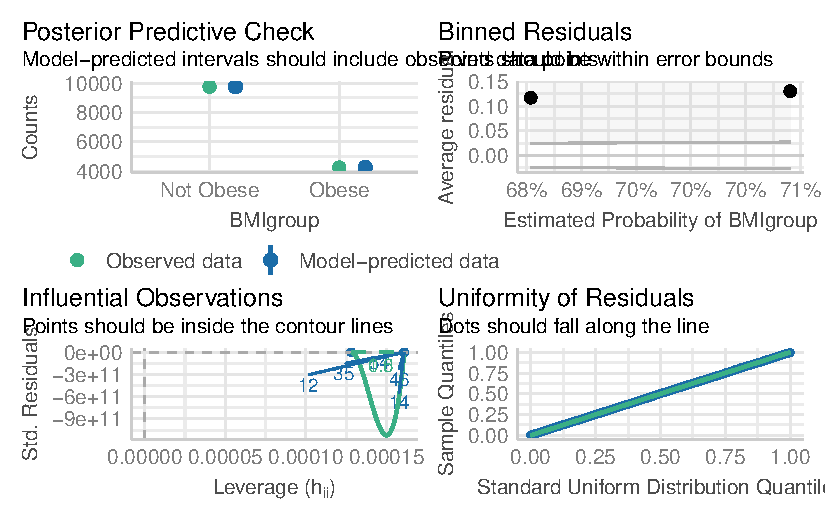
\includegraphics[keepaspectratio]{Data-analysis-12--1---1-_files/figure-pdf/fig-diagnostics2-1.pdf}}

}

\caption{\label{fig-diagnostics2}Diagnostic plots for the sex model}

\end{figure}%

The plots in figure 2 look good enough. There may be issues with the
binned residuals plot, however the issue likely stems from sex being a
factor with 2 levels giving us only 2 points.

We now look at education to consider if there is a difference in obesity
based on socio-economic factors. We fit the following model:

\[
logit(\pi) = \beta_0 + \beta_1 x_i + \beta_2 x_j + \beta_3 x_k + \beta_4 x_l +\beta_5 x_m + \beta_6 x_n + \epsilon_i, ~~~~~ \epsilon_i \sim N(0, \sigma^2), ~~~~~ i = 1, ... , 14017
\] Where \(x_i\) through \(x_n\) are indicator variables taking the
value 1 if they have that level of education and 0 if they do not. The
\(\beta_0\) term refers to the referrence level which is having a
degree.

\begin{longtable}[]{@{}
  >{\centering\arraybackslash}p{(\linewidth - 6\tabcolsep) * \real{0.2500}}
  >{\centering\arraybackslash}p{(\linewidth - 6\tabcolsep) * \real{0.2500}}
  >{\centering\arraybackslash}p{(\linewidth - 6\tabcolsep) * \real{0.2500}}
  >{\centering\arraybackslash}p{(\linewidth - 6\tabcolsep) * \real{0.2500}}@{}}
\toprule\noalign{}
\endhead
\bottomrule\noalign{}
\endlastfoot
~ &
\multicolumn{3}{>{\centering\arraybackslash}p{(\linewidth - 6\tabcolsep) * \real{0.7500} + 4\tabcolsep}@{}}{%
BM Igroup} \\
Predictors & Odds Ratios & CI & p \\
(Intercept) & 3.05 & 2.85~--~3.26 & \textbf{\textless0.001} \\
\begin{minipage}[t]{\linewidth}\raggedright
Education {[}Higher grade\\
or equiv{]}\strut
\end{minipage} & 0.84 & 0.75~--~0.94 & \textbf{0.003} \\
\begin{minipage}[t]{\linewidth}\raggedright
Education {[}HNC/D or\\
equiv{]}\strut
\end{minipage} & 0.72 & 0.64~--~0.82 & \textbf{\textless0.001} \\
\begin{minipage}[t]{\linewidth}\raggedright
Education {[}No\\
qualifications{]}\strut
\end{minipage} & 0.53 & 0.48~--~0.59 & \textbf{\textless0.001} \\
\begin{minipage}[t]{\linewidth}\raggedright
Education {[}Other school\\
level{]}\strut
\end{minipage} & 0.60 & 0.51~--~0.70 & \textbf{\textless0.001} \\
\begin{minipage}[t]{\linewidth}\raggedright
Education {[}Standard grade\\
or equiv{]}\strut
\end{minipage} & 0.67 & 0.60~--~0.74 & \textbf{\textless0.001} \\
R\textsuperscript{2} Tjur &
\multicolumn{3}{>{\raggedright\arraybackslash}p{(\linewidth - 6\tabcolsep) * \real{0.7500} + 4\tabcolsep}@{}}{%
0.011} \\
\end{longtable}

As seen from table 3, all the levels of education are considered
significant predictors of the persons BMI group. The odds of a person
being obese is 3.05 for a person with a degree, then increases by
0.53-0.84 depending on qualification level.

Again, we have to check the model assumptions.

\begin{figure}

\centering{

\pandocbounded{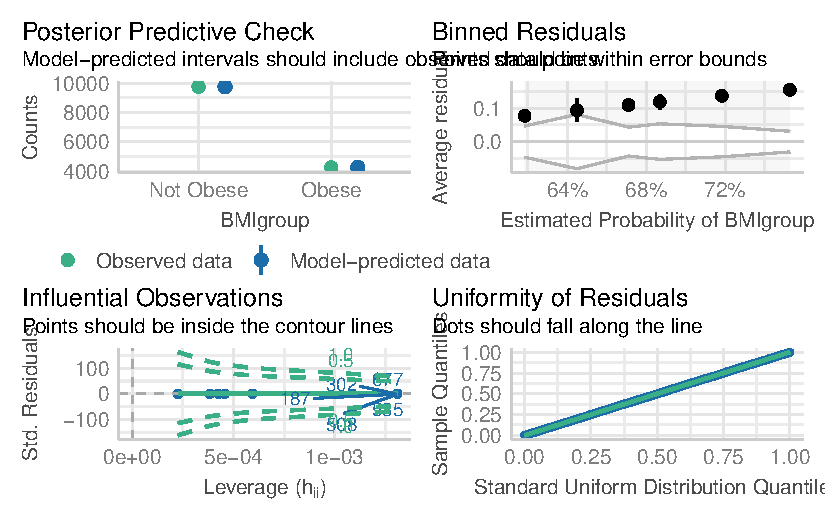
\includegraphics[keepaspectratio]{Data-analysis-12--1---1-_files/figure-pdf/fig-diagnostics3-1.pdf}}

}

\caption{\label{fig-diagnostics3}Diagnostic plots for the education
model}

\end{figure}%

The interpretation of figure 3 is much like the previous figures. The
only graph that leaves cause for concern is the binned residuals graph,
but again, becuase it is a factor, it is always going to not work as
well as a continuous variable. Thus, the model is appropriate.

\subsection{Results}\label{sec-results}

\section{Conclusions}\label{sec-conc}

\begin{quote}
\begin{quote}
\begin{quote}
\begin{quote}
\begin{quote}
\begin{quote}
\begin{quote}
Formal-Analysis-Q2
\end{quote}
\end{quote}
\end{quote}
\end{quote}
\end{quote}
\end{quote}
\end{quote}

From the previous tests, we have seen that age, sex, and education are
all significant in the prediction of an individuals BMI group,
indicating differences in obesity across these factors. As age
increases, the odds of obesity rise. Females have higher odds of being
obese than males, and lower education levels are associated with greater
odds of obesity.




\end{document}
